\documentclass[]{article} 
\usepackage{pgfplots} 
%\usepgfplotslibrary{external} 
%\tikzexternalize 
\usepgfplotslibrary{fillbetween}
\usepackage{tikz} 
\usepackage{amsmath} 
\usepackage{pgfplots} 
\usetikzlibrary{calc} 
\pgfplotsset{compat = newest,every x tick label/.append style={font=\scriptsize,color = white},every y tick label/.append style={font=\scriptsize,color = white}, every axis plot post/.style={line join=round}}

\begin{document} 
	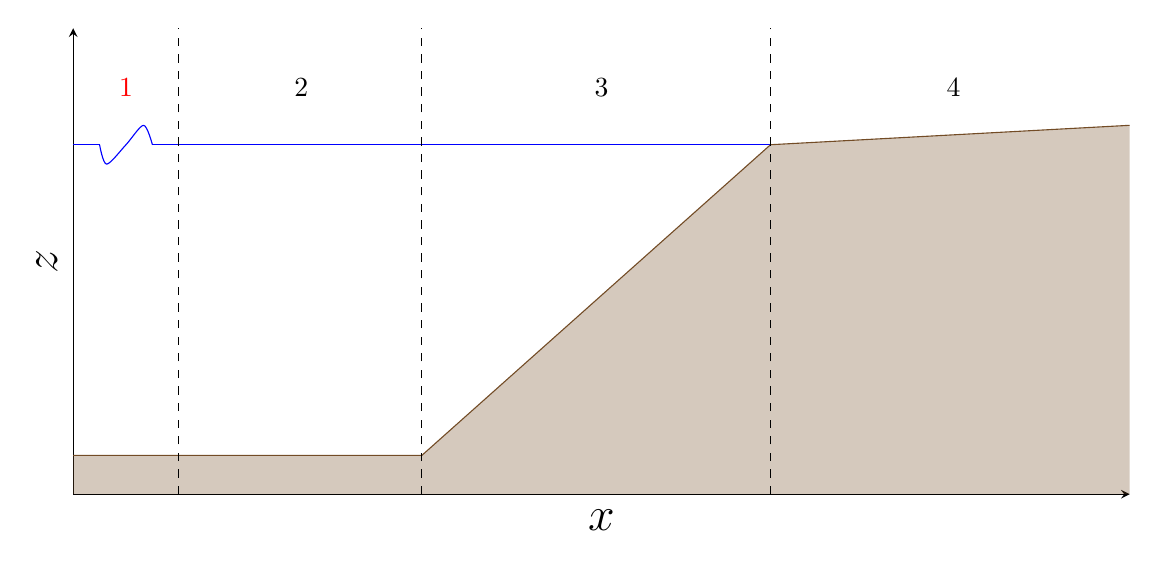
\begin{tikzpicture} 
	\begin{axis}[ 
	width = 0.7\textwidth,
	label style={font=\LARGE},
	axis lines=left, xtick=\empty,
	ytick={-1},
	clip mode=individual,
	xmin=0, 
	xmax=1, 
	width = 15cm,
	height = 7.5cm,
	ymin = -0.1, 
	ymax = 1.1,
	xlabel=$x$, 
	ylabel=$z$ ]
	
	%\draw plot [smooth, blue] coordinates{(0,0.8) (0.025,0.8) (0.03166666666,0.75)  (0.05,0.8) (0.06666666666,0.85)  (0.075,0.8) (0.66,0.8)};
	\addplot [ blue] coordinates {(0,0.8) (0.025,0.8)};
	\addplot [smooth, blue] coordinates {(0.025,0.8) (0.03166666666,0.75)  (0.05,0.8) (0.06666666666,0.85)  (0.075,0.8)};
	\addplot [ blue] coordinates {(0.075,0.8) (0.66,0.8)};
	
    \path[name path=axis] (axis cs:0,-0.1) -- (axis cs:1,-0.1);
    
    \addplot[name path=f, brown!60!black] coordinates {(0,0) (0.33,0) (0.66,0.8) (1,0.85)};
    \addplot [
    thick,
    color=brown!60!black,
    fill=brown!60!black, 
    fill opacity=0.3
    ] fill between[of=f and axis];
	
	
	\node[above] at (0.05,0.9) {\color{red}{1}};
	\addplot [black,dashed] coordinates {(0.1,-0.1) (0.1,1.1)};
	
	\node[above] at (0.216,0.9) {2};
	\addplot [black,dashed] coordinates {(0.33,-0.1) (0.33,1.1)};
	
	\node[above] at (0.5,0.9) {3};
	
	\addplot [black,dashed] coordinates {(0.66,-0.1) (0.66,1.1)};

	\node[above] at (0.8333,0.9) {4};
	
	\end{axis} 
	\end{tikzpicture} 
\end{document}